% CS615 Aspects of System Administration
% Author: Jan Schaumann <jschauma@netmeister.org>
% $Id: slides.tex,v 1.6 2006/03/07 13:55:55 jschauma Exp $

\documentclass[xga]{xdvislides}
\usepackage[landscape]{geometry}
\usepackage{graphics}
\usepackage{graphicx}
\usepackage{colordvi}
\usepackage{fancyvrb}

\fvset{fontfamily=courier,commandchars=\\\{\}}

\begin{document}
\setfontphv

%%% Headers and footers
\lhead{\slidetitle}                               % default:\lhead{\slidetitle}
\chead{CS615 - Aspects of System Administration}% default:\chead{\relax}
\rhead{Slide \thepage}                       % default:\rhead{\sectiontitle}
\lfoot{\Gray{SMTP, Backup and Disaster Recovery}}% default:\lfoot{\slideauthor}
\cfoot{\relax}                               % default:\cfoot{\relax}
\rfoot{\Gray{\today}}

\newcommand{\smallish}{\fontsize{16}{16}\selectfont}

\vspace*{\fill}
\begin{center}
	\Hugesize
		CS615 - Aspects of System Administration\\ [1em]
		SMTP, Backup and Disaster Recovery \\ [1em]
	\hspace*{5mm}\blueline\\ [1em]
	\Normalsize
		Department of Computer Science\\
		Stevens Institute of Technology\\
		Jan Schaumann\\
		\verb+jschauma@stevens-tech.edu+
		\verb+http://www.cs.stevens-tech.edu/~jschauma/615A/+
\end{center}
\vspace*{\fill}

\subsection{Email... still popular}
Bad news, everybody: Slack has not yet replaced email.

\subsection{Email... still popular}
Bad news, everybody: Slack has not yet replaced email.
\\

\begin{itemize}
	\item {\bf 4.6 billion} - number of email accounts.
	\item {\bf 269 billion} - Average number of email messages per day. \\
		That's 3.1 million emails {\em per second}.
	\item {\bf 121} - Average number of emails an office worker receives.
	\item {\bf 42} - Percentage of Americans that check their email in the bathroom.
	\item {\bf 18} - Percentage of Americans that check their email while driving.
	\item {\bf $>$70} - Percentage of emails that are Spam.
\end{itemize}

\subsection{Sending...}
\begin{verbatim}
# tcpdump -i xennet0 -w /tmp/t.out port not 22 2>/dev/null &
# mail -s "CS615 - SMTP Exercise" jschauma@stevens.edu -f jschauma@stevens.edu
Hello,

SMTP is simple.

-Jan
.
EOT
# fg
tcpdump -i xennet0 -w /tmp/t.out port not 22 2>/dev/null
^C
\end{verbatim}


\subsection{Sending...}
\begin{verbatim}
# tail -5 /var/log/maillog
Apr  4 15:42:33 ip-10-235-167-232 postfix/pickup[848]: 2A17275438:
        uid=0 from=<jschauma@stevens.edu>
Apr  4 15:42:33 ip-10-235-167-232 postfix/cleanup[765]: 2A17275438:
        message-id=<20160404154233.2A17275438@ip-10-235-167-232.ec2.internal>
Apr  4 15:42:33 ip-10-235-167-232 postfix/qmgr[876]: 2A17275438:
        from=<jschauma@stevens.edu>, size=380, nrcpt=1 (queue active)
Apr  4 15:42:33 ip-10-235-167-232 postfix/smtp[1124]: 2A17275438:
        to=<jschauma@stevens.edu>, relay=spamfilter01.stevens.edu[155.246.14.37]:25,
        delay=0.62, delays=0.04/0.01/0.03/0.54, dsn=2.0.0,
        status=sent (250 Ok: queued as 688CD6F4001)
Apr  4 15:42:33 ip-10-235-167-232 postfix/qmgr[876]: 2A17275438: removed
\end{verbatim}

\subsection{Sending...}
\begin{verbatim}
# tcpdump -t -r /tmp/t.out port 53
IP 10.235.167.232.65498 > 172.16.0.23.domain: 61195+ MX? stevens.edu. (29)
IP 172.16.0.23.domain > 10.235.167.232.65498: 61195 2/0/0
        MX spamfilter01.stevens.edu. 10,
        MX spamfilter02.stevens.edu. 20 (87)
IP 10.235.167.232.65497 > 172.16.0.23.domain: 1949+
        A? spamfilter01.stevens.edu. (42)
IP 172.16.0.23.domain > 10.235.167.232.65497: 1949 1/0/0 A 155.246.14.37 (58)
IP 10.235.167.232.65496 > 172.16.0.23.domain: 39922+
        AAAA? spamfilter01.stevens.edu. (42)
IP 172.16.0.23.domain > 10.235.167.232.65496: 39922 0/1/0 (113)
IP 10.235.167.232.65495 > 172.16.0.23.domain: 26844+
        A? spamfilter02.stevens.edu. (42)
IP 172.16.0.23.domain > 10.235.167.232.65495: 26844 1/0/0 A 155.246.248.24 (58)
IP 10.235.167.232.65494 > 172.16.0.23.domain: 1439+
        AAAA? spamfilter02.stevens.edu. (42)
IP 172.16.0.23.domain > 10.235.167.232.65494: 1439 0/1/0 (113)
\end{verbatim}

\subsection{Sending...}
\begin{verbatim}
# host -t mx stevens.edu
stevens.edu mail is handled by 20 spamfilter02.stevens.edu.
stevens.edu mail is handled by 10 spamfilter01.stevens.edu.
# host spamfilter01.stevens.edu.
spamfilter01.stevens.edu has address 155.246.14.37
# host spamfilter02.stevens.edu.
spamfilter02.stevens.edu has address 155.246.248.24
#
\end{verbatim}

\subsection{Sending...}
\smallish
\begin{verbatim}
IP 10.235.167.232.65524 > 155.246.14.37.smtp: Flags [S], seq 1528496417,
IP 155.246.14.37.smtp > 10.235.167.232.65524: Flags [S.], seq 3510048077, ack 1528496418
IP 10.235.167.232.65524 > 155.246.14.37.smtp: Flags [.], ack 1, 
IP 155.246.14.37.smtp > 10.235.167.232.65524: Flags [P.], seq 1:72, ack 1, length 71
IP 10.235.167.232.65524 > 155.246.14.37.smtp: Flags [P.], seq 1:38, ack 72, length 37
IP 155.246.14.37.smtp > 10.235.167.232.65524: Flags [.], ack 38, 
IP 155.246.14.37.smtp > 10.235.167.232.65524: Flags [P.], seq 72:244, ack 38, length 172
IP 10.235.167.232.65524 > 155.246.14.37.smtp: Flags [P.], seq 38:119, ack 244, length 81
IP 155.246.14.37.smtp > 10.235.167.232.65524: Flags [P.], seq 244:282, ack 119, length 38
IP 10.235.167.232.65524 > 155.246.14.37.smtp: Flags [.], ack 282,
IP 155.246.14.37.smtp > 10.235.167.232.65524: Flags [P.], seq 282:369, ack 119, length 87
IP 10.235.167.232.65524 > 155.246.14.37.smtp: Flags [P.], seq 119:508, ack 369, length 389
IP 155.246.14.37.smtp > 10.235.167.232.65524: Flags [.], ack 508
IP 155.246.14.37.smtp > 10.235.167.232.65524: Flags [P.], seq 369:400, ack 508, length 31
IP 155.246.14.37.smtp > 10.235.167.232.65524: Flags [FP.], seq 400:499, ack 508, length 99
IP 10.235.167.232.65524 > 155.246.14.37.smtp: Flags [.], ack 500
IP 10.235.167.232.65524 > 155.246.14.37.smtp: Flags [F.], seq 508, ack 500
IP 155.246.14.37.smtp > 10.235.167.232.65524: Flags [.], ack 509
\end{verbatim}
\Normalsize

\subsection{Sending...}
\begin{Verbatim}
$ telnet 155.246.14.37 25
Trying 155.246.14.37...
Connected to spamfilter01.stevens.edu.
Escape character is '^]'.
\textbf{220 spamfilter01.stevens.edu ESMTP (fe32969a29a5f461e53bf93b18c8fdb5)}
EHLO ip-10-235-167-232.ec2.internal
\textbf{250-spamfilter01.stevens.edu Hello ec2-54-205-68-41.compute-1.amazonaws.com [54.205.68.41],}
\textbf{        pleased to meet you}
\textbf{250-SIZE 50000000}
\textbf{250-PIPELINING}
\textbf{250-8BITMIME}
\textbf{250 HELP}
MAIL FROM:<jschauma@stevens.edu> SIZE=380
\textbf{250 Sender <jschauma@stevens.edu> OK}
RCPT TO:<jschauma@stevens.edu>
\textbf{250 Recipient <jschauma@stevens.edu> OK}
\end{Verbatim}

\subsection{Sending...}
\begin{Verbatim}
DATA
\textbf{354 Start mail input; end with <CRLF>.<CRLF>}
Received: by ip-10-235-167-232.ec2.internal (Postfix, from userid 0)
        id 2A17275438; Mon,  4 Apr 2016 15:42:33 +0000 (UTC)
To: jschauma@stevens.edu
Subject: CS615 - SMTP Exercise
Message-Id: <20160404154233.2A17275438@ip-10-235-167-232.ec2.internal>
Date: Mon,  4 Apr 2016 15:42:33 +0000 (UTC)
From: jschauma@stevens.edu (Charlie Root)

Hello,

SMTP is simple.

-Jan
.
\textbf{250 Ok: queued as 6A9C76F4004}
\end{Verbatim}

\subsection{SMTP Codes}
SMTP codes consist of three digits in five classes:
\begin{itemize}
	\item {\bf 1xx} --  Mail server has accepted the command, but does not yet
		take any action. A confirmation message is required.
	\item {\bf 2xx} --  Mail server has completed the task successfully
		without errors.
	\item {\bf 3xx} --  Mail server has understood the request, but requires
		further information to complete it.
	\item {\bf 4xx} --  Mail server has encountered a temporary failure. If
		the command is repeated without any change, it might be
		completed. Try again, it may help!
	\item {\bf 5xx} --  Mail server has encountered a fatal error. Your
		request can't be processed.
\end{itemize}

\subsection{Receiving...}
\begin{verbatim}
Date: Mon, 4 Apr 2016 15:42:33 +0000
From: jschauma@stevens.edu (Charlie Root)
To: Jan Schaumann <jschauma@stevens.edu>
Subject: CS615 - SMTP Exercise

Hello,

SMTP is simple.

-Jan
\end{verbatim}

\subsection{Receiving...}
\smallish
\begin{verbatim}
From jschauma@stevens.edu  Mon Apr  4 11:42:35 2016
Received: by panix.netmeister.org (Postfix, from userid 1004)
        id 6B0F56513D; Mon,  4 Apr 2016 11:42:35 -0400 (EDT)
Received: from nexus.stevens.edu (nexus.stevens.edu [155.246.14.12])
        by panix.netmeister.org (Postfix) with ESMTP id 2AD596513B
Received: from exchng02.campus.stevens-tech.edu (exchng02.campus.stevens-tech.edu [155.246.14.23])
        by nexus.stevens.edu (Postfix) with ESMTPS id 11E3817F825
Received: from exchng04.campus.stevens-tech.edu (2002:9bf6:f826::9bf6:f826) by
        exchng02.campus.stevens-tech.edu (2002:9bf6:e17::9bf6:e17) with Microsoft
        SMTP Server (TLS) id 15.0.1104.5; Mon, 4 Apr 2016 11:42:34 -0400
Received: from exchng03.campus.stevens-tech.edu (155.246.248.36) by
        exchng04.campus.stevens-tech.edu (155.246.248.39) with Microsoft SMTP Server
        (TLS) id 15.0.1104.5; Mon, 4 Apr 2016 11:42:34 -0400
Received: from exchng03.campus.stevens-tech.edu ([::1]) by
        exchng03.campus.stevens-tech.edu ([fe80::599a:f128:d1b3:4ce7%12]) with
        Microsoft SMTP Server id 15.00.1104.000; Mon, 4 Apr 2016 11:42:34 -0400
From: Jan Schaumann <jschauma@stevens.edu>
To: Jan Schaumann <jschauma@stevens.edu>
Subject: CS615 - SMTP Exercise
Date: Mon, 4 Apr 2016 15:42:33 +0000
Message-ID: <1b1399e9c44b494f99e9d0030f0fa74b@exchng03.campus.stevens-tech.edu>
x-barracuda-apparent-source-ip: 54.205.68.41
x-ms-exchange-parent-message-id: <20160404154233.2A17275438@ip-10-235-167-232.ec2.internal>
Resent-Message-Id: <20160404154235.11E3817F825@nexus.stevens.edu>
\end{verbatim}

\subsection{Receiving...}
\begin{verbatim}
$ tail -f /var/log/maillog
postfix/smtpd[552]: connect from nexus.stevens.edu[155.246.14.12]
postfix/smtpd[552]: 2AD596513B: client=nexus.stevens.edu[155.246.14.12]
postfix/cleanup[6975]: 2AD596513B:
        message-id=<1b1399e9c44b494f99e9d0030f0fa74b@exchng03.campus.stevens-tech.edu>
postfix/cleanup[6975]: 2AD596513B:
        resent-message-id=<20160404154235.11E3817F825@nexus.stevens.edu>
postfix/smtpd[552]: disconnect from nexus.stevens.edu[155.246.14.12]
postfix/qmgr[24644]: 2AD596513B: from=<jschauma@stevens.edu>, size=3116, nrcpt=1 (queue active)
spamd[24829]: spamd: connection from localhost [::1]:58531 to port 783, fd 5
spamd: processing message <1b1399e9c44b494f99e9d0030f0fa74b@exchng03.campus.stevens-tech.edu>
        aka <20160404154235.11E3817F825@nexus.stevens.edu> for spamd:1004
postfix/pipe[8278]: 2AD596513B: to=<jschauma@netmeister.org>, relay=spamassassin, delay=0.29,
        delays=0.05/0.01/0/0.23, dsn=2.0.0, status=sent (delivered via spamassassin service)
postfix/qmgr[24644]: 2AD596513B: removed
postfix/pickup[16387]: 6B0F56513D: uid=1004 from=<jschauma@stevens.edu>
postfix/cleanup[6975]: 6B0F56513D:
        message-id=<1b1399e9c44b494f99e9d0030f0fa74b@exchng03.campus.stevens-tech.edu>
postfix/cleanup[6975]: 6B0F56513D:
        resent-message-id=<20160404154235.11E3817F825@nexus.stevens.edu>
postfix/qmgr[24644]: 6B0F56513D: from=<jschauma@stevens.edu>, size= 3442, nrcpt=1 (queue active)
postfix/local[2264]: 6B0F56513D: to=<jschauma@netmeister.org>, relay=local,
        delay=0.15, delays=0.08/0.01/0/0.06, dsn=2.0.0, status=sent (delivered to command:
        /usr/pkg/bin/procmail)
\end{verbatim}
\Normalsize

\subsection{Receiving...}
\begin{verbatim}
IP 155.246.14.12.37547 > 166.84.7.99.25: Flags [S], seq 2435028943
IP 166.84.7.99.25 > 155.246.14.12.37547: Flags [S.], seq 4137148947, ack 2435028944
IP 155.246.14.12.37547 > 166.84.7.99.25: Flags [.], ack 1
IP 166.84.7.99.51798 > 166.84.67.2.53: 29782+ PTR? 12.14.246.155.in-addr.arpa. (44)
IP 166.84.67.2.53 > 166.84.7.99.51798: 29782 1/2/2 PTR nexus.stevens.edu. (160)
IP 166.84.7.99.51797 > 166.84.67.2.53: 17361+ A? nexus.stevens.edu. (35)
IP 166.84.67.2.53 > 166.84.7.99.51797: 17361 1/3/3 A 155.246.14.12 (173)
\end{verbatim}

\subsection{Receiving...}
\begin{verbatim}
IP 166.84.7.99.25 > 155.246.14.12.37547: Flags [P.], seq 1:41, ack 1
IP 155.246.14.12.37547 > 166.84.7.99.25: Flags [.], ack 41
IP 155.246.14.12.37547 > 166.84.7.99.25: Flags [P.], seq 1:25, ack 41
IP 166.84.7.99.25 > 155.246.14.12.37547: Flags [P.], seq 41:174, ack 25
IP 155.246.14.12.37547 > 166.84.7.99.25: Flags [P.], seq 25:157, ack 174
IP 166.84.7.99.51796 > 166.84.67.2.53: 41349+ MX? stevens.edu. (29)
IP 166.84.67.2.53 > 166.84.7.99.51796: 41349 2/3/5 MX spamfilter02.stevens.edu.
      20, MX spamfilter01.stevens.edu. 10 (241)
IP 166.84.7.99.51795 > 166.84.67.2.53: 51732+ A? nexus.stevens.edu. (35)
IP 166.84.67.2.53 > 166.84.7.99.51795: 51732 1/3/3 A 155.246.14.12 (173)
IP 166.84.7.99.51794 > 166.84.67.2.53: 64776+ A? 12.14.246.155.sbl.spamhaus.org. (48)
IP 166.84.67.2.53 > 166.84.7.99.51794: 64776 NXDomain 0/1/0 (112)
\end{verbatim}


\subsection{Receiving...}
\begin{verbatim}
IP 166.84.7.99.25 > 155.246.14.12.37547: Flags [P.], seq 174:239, ack 157
IP 155.246.14.12.37547 > 166.84.7.99.25: Flags [.], seq 157:1605, ack 239
IP 155.246.14.12.37547 > 166.84.7.99.25: Flags [.], seq 1605:3053, ack 239
IP 155.246.14.12.37547 > 166.84.7.99.25: Flags [P.], seq 3053:3080, ack 239
IP 166.84.7.99.25 > 155.246.14.12.37547: Flags [.], ack 3053, win 4016,
IP 166.84.7.99.25 > 155.246.14.12.37547: Flags [P.], seq 239:290, ack 3080
IP 166.84.7.99.25 > 155.246.14.12.37547: Flags [F.], seq 290, ack 3080
IP 155.246.14.12.37547 > 166.84.7.99.25: Flags [F.], seq 3080, ack 290
IP 166.84.7.99.25 > 155.246.14.12.37547: Flags [.], ack 3081, win 4197
IP 155.246.14.12.37547 > 166.84.7.99.25: Flags [.], ack 291, win 123
\end{verbatim}

\subsection{Receiving...}
\small
\begin{verbatim}
IP 166.84.7.99.50935 > 166.84.67.2.53: 12067 [1au] A? 12.14.246.155.psbl.surriel.com. (59)
IP 166.84.7.99.50935 > 166.84.67.2.53: 39395 [1au] A? 12.14.246.155.bb.barracudacentral.org. (66)
IP 166.84.7.99.50935 > 166.84.67.2.53: 17365 [1au] A? 12.14.246.155.bl.score.senderscore.com. (67)
IP 166.84.7.99.50935 > 166.84.67.2.53: 38635 [1au] TXT? 37.248.246.155.bl.spamcop.net. (58)
IP 166.84.7.99.50935 > 166.84.67.2.53: 10907 [1au] TXT? 21.14.246.155.bl.spamcop.net. (57)
IP 166.84.7.99.50935 > 166.84.67.2.53: 11246 [1au] TXT? 12.14.246.155.bl.spamcop.net. (57)
IP 166.84.67.2.53 > 166.84.7.99.50935: 39395 0/2/7 (206)
IP 166.84.67.2.53 > 166.84.7.99.50935: 12067 0/4/6 (247)
IP 166.84.67.2.53 > 166.84.7.99.50935: 17365 0/4/5 (254)
IP 166.84.67.2.53 > 166.84.7.99.50935: 38635 0/8/9 (354)
IP 166.84.67.2.53 > 166.84.7.99.50935: 13318 0/8/9 (403)
IP 166.84.67.2.53 > 166.84.7.99.50935: 10907 0/8/9 (353)
IP 166.84.7.99.50935 > 166.84.67.2.53: 8582 [1au] A? 37.248.246.155.dnsbl.sorbs.net. (59)
IP 166.84.7.99.50935 > 166.84.67.2.53: 61203 [1au] A? 21.14.246.155.dnsbl.sorbs.net. (58)
IP 166.84.7.99.50935 > 166.84.67.2.53: 59454 [1au] A? 12.14.246.155.dnsbl.sorbs.net. (58)
IP 166.84.7.99.50935 > 166.84.67.2.53: 7289 [1au] A? 12.14.246.155.iadb.isipp.com. (57)
IP 166.84.7.99.50935 > 166.84.67.2.53: 63596 [1au] TXT? 12.14.246.155.sa-trusted.bondedsender.org. (70)
IP 166.84.7.99.50935 > 166.84.67.2.53: 18732 [1au] TXT? 12.14.246.155.sa-accredit.habeas.com.
(65)
IP 166.84.7.99.50935 > 166.84.67.2.53: 43600 [1au] A? 12.14.246.155.bl.mailspike.net. (59)
IP 166.84.67.2.53 > 166.84.7.99.50935: 49122 0/19/80 (1472)
IP 166.84.67.2.53 > 166.84.7.99.50935: 6461 0/6/10 (360)
IP 166.84.67.2.53 > 166.84.7.99.50935: 54452 0/13/14 (607)
IP 166.84.67.2.53 > 166.84.7.99.50935: 8582 0/13/14 (558)
IP 166.84.67.2.53 > 166.84.7.99.50935: 61203 0/13/14 (557)
IP 166.84.67.2.53 > 166.84.7.99.50935: 59454 0/13/14 (557)
IP 166.84.67.2.53 > 166.84.7.99.50935: 7289 0/5/7 (288)
IP 166.84.67.2.53 > 166.84.7.99.50935: 63596 0/18/19 (879)
IP 166.84.67.2.53 > 166.84.7.99.50935: 18732 0/15/16 (742)
IP 166.84.67.2.53 > 166.84.7.99.50935: 43600 0/2/3 (126)
IP 166.84.7.99.50935 > 166.84.67.2.53: 2649 [1au] TXT? nexus.stevens.edu. (46)
IP 166.84.67.2.53 > 166.84.7.99.50935: 2649 0/3/4 (168)
\end{verbatim}
\Normalsize

\subsection{Relaying mail}
\begin{verbatim}
$ telnet spamfilter01.stevens.edu 25
Trying 155.246.14.37...
Connected to spamfilter01.stevens.edu.
Escape character is '^]'.
220 spamfilter01.stevens.edu ESMTP (fe32969a29a5f461e53bf93b18c8fdb5)
ehlo localhost
250-spamfilter01.stevens.edu Hello ec2-54-205-68-41.compute-1.amazonaws.com
        [54.205.68.41], pleased to meet you
250-SIZE 50000000
250-PIPELINING
250-8BITMIME
250 HELP
MAIL FROM:<obama@whitehouse.gov>
250 Sender <obama@whitehouse.gov> OK
RCPT TO:<comey@fbi.gov>
550 No such domain at this location
\end{verbatim}

\subsection{Authenticity}
\begin{verbatim}
MAIL FROM:<obama@whitehouse.gov>
250 Sender <obama@whitehouse.gov> OK
RCPT TO:<jschauma@stevens-tech.edu>
250 Recipient <jschauma@stevens-tech.edu> OK
DATA
354 Start mail input; end with <CRLF>.<CRLF>
From: "Barack Obama" <obama@whitehouse.gov>
Subject: Friday

Yo,

Party at my house.
BYOB.

-B
.
250 Ok: queued as 61D4D6F4003
\end{verbatim}

\subsection{Authenticity}
\begin{verbatim}
MAIL FROM:<president@stevens.edu>
250 Sender <president@stevens.edu> OK
RCPT TO:<jschauma@stevens-tech.edu>
250 Recipient <jschauma@stevens-tech.edu> OK
DATA
354 Start mail input; end with <CRLF>.<CRLF>
From: "Barack Obama" <obama@whitehouse.gov>
Subject: Friday

Yo,

Party at my house.
BYOB.

-B
.
250 Ok: queued as 61D4D6F4003
\end{verbatim}

\subsection{Authenticity}
\begin{verbatim}
Date: Mon,  4 Apr 2016 15:35:12 -0400 (EDT)
From: Barack Obama <obama@whitehouse.gov>
To: undisclosed-recipients: ;
Subject: Friday

Yo,

Party at my house.
BYOB.

-B
\end{verbatim}

\subsection{Authenticity}
\begin{verbatim}
From president@stevens.edu  Mon Apr  4 15:35:12 2016                                                
Return-Path: <president@stevens.edu>                                                                
Date: Mon,  4 Apr 2016 15:35:12 -0400 (EDT)
From: Barack Obama <obama@whitehouse.gov>
To: undisclosed-recipients: ;
Subject: Friday

Yo,

Party at my house.
BYOB.

-B
\end{verbatim}

\subsection{SMTP is a Simple Mail Transfer Protocol.}

\begin{itemize}
	\item TCP port 25
	\item DNS MX records
	\item mail may be relayed or processed by many servers in transit
	\item transport is in clear text
	\item STARTTLS may provide (opportunistic) transport encryption
	\item SPAM controls may include DNS lookups, bayesian scoring, ...
	\item authenticity not guaranteed
\end{itemize}

\subsection{The Mail System}
Divided into:
\begin{itemize}
	\item {\em Mail User Agent} or MUA, such as {\tt mutt(1)}, {\em Mail.app}, {\em Outlook}, a browser (ugh) ...
	\item {\em Mail Transfer Agent} or MTA, such as {\em postfix},
		{\em sendmail}, {\em qmail}, ...
	\item {\em Mail Delivery Agent} or MDA, such as {\em procmail}
	\item {\em Access Agent} providing access via {\em POP}, {\em IMAP} etc.
\end{itemize}

\subsection{Anatomy of an email message}
An email consists of:
\begin{itemize}
	\item mandatory headers (such as "From ", "Delivered-To: ", ...)
	\item optional headers (such as "From: ", "To: ", "Subject: ", ...)
	\item the (optional) body of the message
\end{itemize}

\subsection{Service Considerations}
\begin{itemize}
	\item outsourcing versus in-house
	\item privacy considerations
	\item spam protections
	\item phishing protections
	\item mail delivery cannons for notifications vs. spam lists
	\item high volume traffic demands fine-tuned systems
	\item high volume traffic implications on logging
\end{itemize}
\vspace{.5in}
See also:
\begin{itemize}
	\item {\tt http://is.gd/JQp1zM}
	\item {\tt http://is.gd/cXyrwX}
	\item {\tt http://is.gd/o6Y5f8}
\end{itemize}

\newpage
\vspace*{\fill}
\begin{center}
    \Hugesize
        Hooray! \\ [1em]
    \hspace*{5mm}
    \blueline\\
    \hspace*{5mm}\\
        5 Minute Break
\end{center}
\vspace*{\fill}

\subsection{Know a Unix Command}
\vspace*{\fill}
\begin{center}
	
\includegraphics[scale=0.9]{pics/tar.eps} \\
	\verb+https://www.xkcd.com/1168/+ \\
	\verb+https://www.cs.stevens.edu/~jschauma/615/tar.html+
\end{center}
\vspace*{\fill}

\subsection{Backups}
\begin{itemize}
	\item backup vs. restore
\end{itemize}

\subsection{Backups}
\begin{itemize}
	\item backup vs. restore
	\item backup devices and media
\end{itemize}
\vspace*{\fill}
\begin{center}
	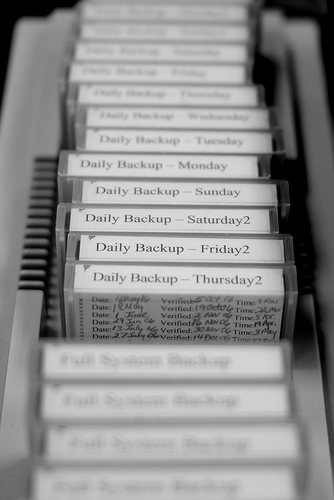
\includegraphics[scale=2.0]{pics/daily-tapes.eps}
\end{center}
\vspace*{\fill}

\subsection{Backups}
\begin{itemize}
	\item backup vs. restore
	\item backup devices and media
\end{itemize}
\vspace*{\fill}
\begin{center}
	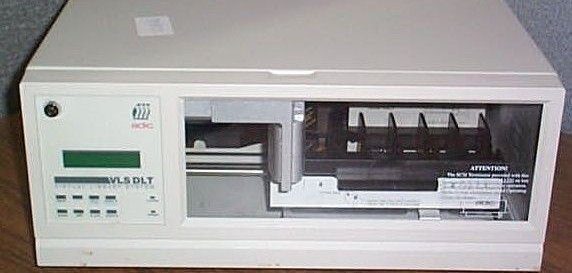
\includegraphics[scale=0.8]{pics/dlt-library.eps}
\end{center}
\vspace*{\fill}

\subsection{Backups}
\begin{itemize}
	\item backup vs. restore
	\item backup devices and media
\end{itemize}
\vspace*{\fill}
\begin{center}
	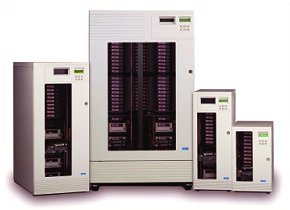
\includegraphics[scale=1.0]{pics/libraries.eps}
\end{center}
\vspace*{\fill}

\subsection{Backups}
\begin{itemize}
	\item backup vs. restore
	\item backup devices and media
	\item filesystem considerations
\end{itemize}

\subsection{Backups}
\begin{itemize}
	\item backup vs. restore
	\item backup devices and media
	\item filesystem considerations
	\item backup strategies
\end{itemize}

\subsection{Backups}
\begin{itemize}
	\item backup vs. restore
	\item backup devices and media
	\item filesystem considerations
	\item backup strategies
	\item planning for disasters
\end{itemize}

\subsection{Backups and Restore Basics}
When do we need backups?

\subsection{Backups and Restore Basics}
When do we need backups?
\begin{itemize}
	\item disaster recovery: off-site storage of sensitive data
	\item long-term storage requirements
	\item recover from data loss
\end{itemize}

\subsection{Backups and Restore Basics}
When do we need backups?
\begin{itemize}
	\item disaster recovery: off-site storage of sensitive data
	\item long-term storage requirements
	\item recover from data loss due to
\end{itemize}
\vspace*{\fill}
\begin{center}
	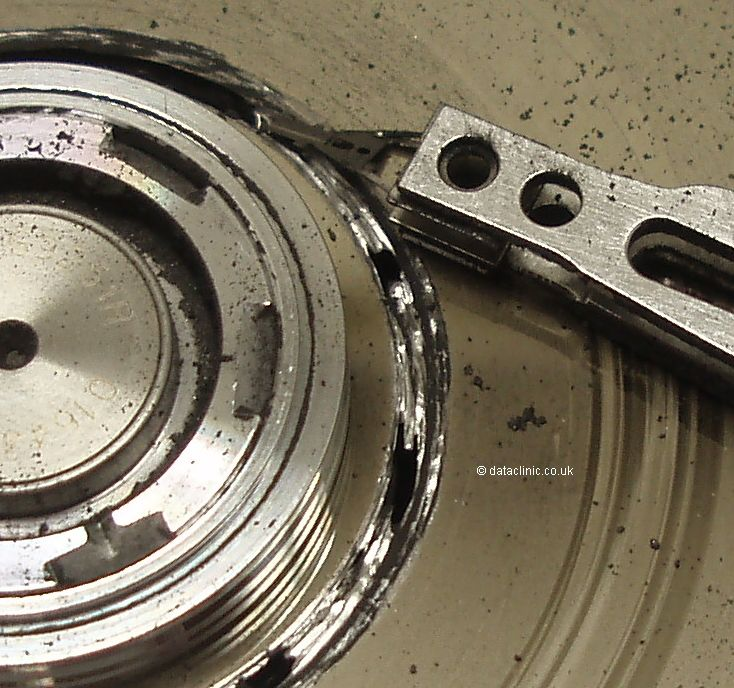
\includegraphics[scale=1.0]{pics/headcrash-closeup.eps}
\end{center}
\vspace*{\fill}

\subsection{Backups and Restore Basics}
When do we need backups?
\begin{itemize}
	\item disaster recovery: off-site storage of sensitive data
	\item long-term storage requirements
	\item recover from data loss due to
\end{itemize}
\vspace*{\fill}
\begin{center}
	
\includegraphics[scale=1.2]{pics/dumb-user.eps}
\end{center}
\vspace*{\fill}

\subsection{Backups and Restore Basics}
When do we need backups?
\begin{itemize}
	\item disaster recovery: off-site storage of sensitive data
	\item long-term storage requirements
	\item recover from data loss due to
\end{itemize}
\vspace*{\fill}
\begin{center}
	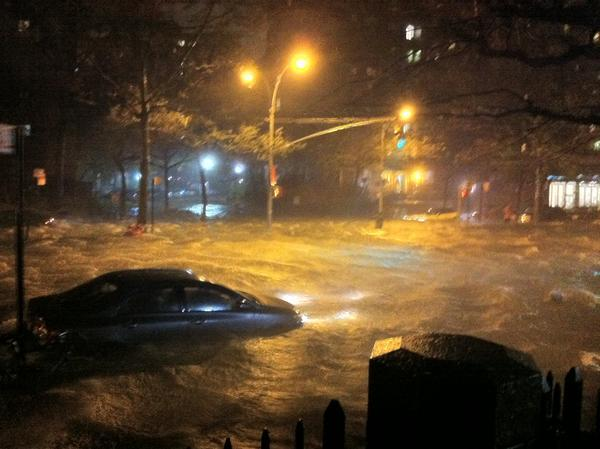
\includegraphics[scale=0.4]{pics/20th-and-C.eps}
\end{center}
\vspace*{\fill}

\subsection{Backups and Restore Basics}
When do we need backups?
\begin{itemize}
	\item disaster recovery: off-site storage of sensitive data
	\item long-term storage requirements
	\item recover from data loss due to
\end{itemize}
\vspace*{\fill}
\begin{center}
	
\includegraphics[scale=0.6]{pics/hacker.eps}
\end{center}
\vspace*{\fill}

\subsection{Backups and Restore Basics}
When do we need backups?
\begin{itemize}
	\item disaster recovery: off-site storage of sensitive data
	\item long-term storage requirements
	\item recover from data loss due to
\end{itemize}
\vspace*{\fill}
\begin{center}
	
\includegraphics[scale=0.6]{pics/bugs.eps}
\end{center}
\vspace*{\fill}

\subsection{Backups and Restore Basics}
When do we need backups?
\begin{itemize}
	\item disaster recovery: off-site storage of sensitive data
	\item long-term storage requirements
	\item recover from data loss due to
		\begin{itemize}
			\item equipment failure
			\item bozotic users
			\item natural disaster
			\item security breach
			\item software bugs
		\end{itemize}
\end{itemize}

\subsection{Backups and Restore Basics}
When do we need backups?
\begin{itemize}
	\item disaster recovery: off-site storage of sensitive data
	\item long-term storage requirements
	\item recover from data loss due to
		\begin{itemize}
			\item equipment failure
			\item bozotic users
			\item natural disaster
			\item security breach
			\item software bugs
		\end{itemize}
\end{itemize}
\addvspace{.5in}
Think of your backups as {\em insurance}:  you invest and pay for it, hoping
you will never need it.


\subsection{Key Reasons for Restores}
Three key reasons for restores: {\em Accidental File Deletion}, {\em Disk
Failure} and {\em Archival}.
\\

1. Accidental File Deletion
\begin{itemize}
	\item ability to restore a file within a certain time frame
	\item restore time, including
		\begin{itemize}
			\item actual time spent restoring
			\item waiting until resources permit the restore
			\item staff availability
		\end{itemize}
	\item self-service restore
\end{itemize}

\subsection{Key Reasons for Restores}
2. Disk Failure
\begin{itemize}
	\item loss of entire file system
	\item leads to downtime
	\item RAID may help
	\item takes long time to restore
\end{itemize}
\addvspace{.5in}
3. Archival
\begin{itemize}
	\item {\em full} set of level 0 backups
	\item separate set from regular backups
	\item usually stored off-site
	\item store for long time
\end{itemize}

\subsection{Filesystem backup}
{\tt dump(8)} / {\tt restore(8)}
\begin{itemize}
	\item in use since \~{}1975
	\item full filesystem level backups
	\item direct interaction with tape devices
	\item integration with {\tt /etc/fstab}
	\item efficient incremental backups
\end{itemize}

\subsection{Filesystem backup}
\begin{itemize}
	\item start an EC2 instance
	\item create a full filesystem backup using \verb+dump(8)+
	\item add e.g. the 'apache' package
	\item create an incremental backup
	\item delete the 'apache' package
	\item restore all files from the incremental backup using the \verb+restore(8)+ command
	\item verify that the 'apache' package is fully installed
\end{itemize}

\subsection{Filesystem backup}
\smallish
\begin{verbatim}
ssh ec2-instance "sudo dump -u -0 -f - /" | bzip2 -c -9 >tmp/ec2.0.bz2
  DUMP: Date of this level 0 dump: Thu Mar 26 19:25:06 2015
  DUMP: Dumping /dev/xvda1 (/) to standard output
  DUMP: Label: cloudimg-rootfs
  DUMP: Writing 10 Kilobyte records
  DUMP: mapping (Pass I) [regular files]
  DUMP: mapping (Pass II) [directories]
  DUMP: estimated 823759 blocks.
  DUMP: Volume 1 started with block 1 at: Thu Mar 26 19:25:07 2015
  DUMP: dumping (Pass III) [directories]
  DUMP: dumping (Pass IV) [regular files]
  DUMP: Volume 1 completed at: Thu Mar 26 19:28:21 2015
  DUMP: Volume 1 820690 blocks (801.46MB)
  DUMP: Volume 1 took 0:03:14
  DUMP: Volume 1 transfer rate: 4230 kB/s
  DUMP: 820690 blocks (801.46MB)
  DUMP: finished in 194 seconds, throughput 4230 kBytes/sec
  DUMP: Date of this level 0 dump: Thu Mar 26 19:25:06 2015
  DUMP: Date this dump completed:  Thu Mar 26 19:28:21 2015
  DUMP: Average transfer rate: 4230 kB/s
  DUMP: DUMP IS DONE
\end{verbatim}
\Normalsize


\subsection{Filesystem backup}
\smallish
\begin{verbatim}
$ cat /var/lib/dumpdates 
/dev/xvda1 0 Thu Mar 26 19:25:06 2015 +0000
$ sudo apt-get install apache2
[...]
$ ssh ec2-instance "sudo dump -u -i -f - /" | bzip2 -c -9 >tmp/ec2.1.bz2
  DUMP: Date of this level i dump: Thu Mar 26 19:56:45 2015
  DUMP: Date of last level 0 dump: Thu Mar 26 19:48:58 2015
  DUMP: Dumping /dev/xvda1 (/) to standard output
  DUMP: Writing 10 Kilobyte records
  DUMP: mapping (Pass I) [regular files]
  DUMP: mapping (Pass II) [directories]
  DUMP: estimated 39644 blocks.
  DUMP: Volume 1 started with block 1 at: Thu Mar 26 19:56:50 2015
  DUMP: dumping (Pass III) [directories]
  DUMP: dumping (Pass IV) [regular files]
  DUMP: Volume 1 completed at: Thu Mar 26 19:56:56 2015
  DUMP: Volume 1 39820 blocks (38.89MB)
  DUMP: Volume 1 transfer rate: 6636 kB/s
  DUMP: 39820 blocks (38.89MB)
  DUMP: finished in 5 seconds, throughput 7964 kBytes/sec
  DUMP: Date of this level i dump: Thu Mar 26 19:56:45 2015
  DUMP: Date this dump completed:  Thu Mar 26 19:56:56 2015
  DUMP: Average transfer rate: 6636 kB/s
  DUMP: DUMP IS DONE
\end{verbatim}
\Normalsize

\subsection{Filesystem backup}
\vspace*{\fill}
\begin{center}
	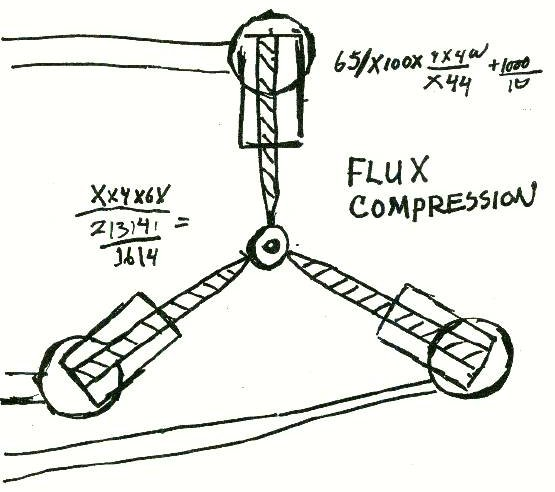
\includegraphics[scale=0.7]{pics/flux-capacitor.eps}
\end{center}
\vspace*{\fill}

\subsection{Filesystem backup}
\vspace*{\fill}
\begin{center}
	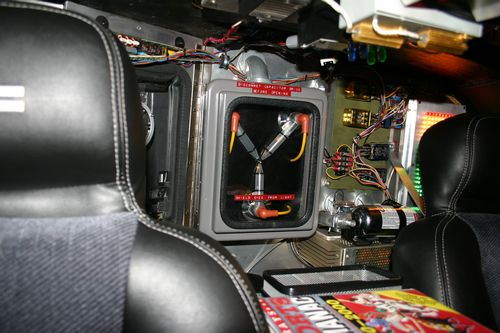
\includegraphics[scale=2.5]{pics/flux-capacitor2.eps}
\end{center}
\vspace*{\fill}

\subsection{Filesystem backup}
\vspace*{\fill}
\begin{center}
	
\includegraphics[scale=0.6]{pics/Time_Machine.eps}
\end{center}
\vspace*{\fill}


\subsection{Filesystem backup}
Example: Mac OS X ``Time Machine'':
\begin{itemize}
	\item automatically creates a full backup (equivalent of a "level 0 dump")
		to separate device or NAS, recording (specifically) last-modified date
		of all directories
	\item every hour, creates a full copy via {\em hardlinks} (hence no
		additional disk space consumed) for files that have not changed,
		new copy of files that have changed
		\item changed files are determined by inspecting last-modified date of
			directories (cheaper than doing comparison of all files'
			last-modified date or data)
	\item saves hourly backups for 24 hours, daily backups for
		the past month, and weekly backups for everything older than a month.
\end{itemize}

\subsection{Filesystem backup}
Example: WAFL (Write Anywhere File Layout)
\begin{itemize}
	\item used by NetApp's ``Data ONTAP'' OS
	\item a snapshot is a read-only copy of a file system (cheap and near
		instantaneous, due to CoW)
	\item uses regular snapshots (``consistency points'', every 10 seconds)
		to allow for speedy recovery from crashes
\end{itemize}
\vspace*{\fill}
\begin{center}
	
\includegraphics[scale=0.75]{pics/waffles.eps}
\end{center}
\vspace*{\fill}


\subsection{Filesystem backup}
Example: WAFL (Write Anywhere File Layout)
\vspace*{\fill}
\begin{center}
	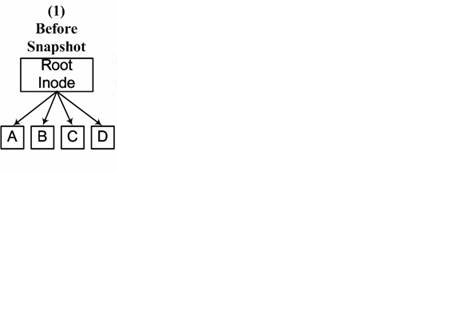
\includegraphics[scale=1.0]{pics/wafl0.eps}
\end{center}
\vspace*{\fill}


\subsection{Filesystem backup}
Example: WAFL (Write Anywhere File Layout)
\vspace*{\fill}
\begin{center}
	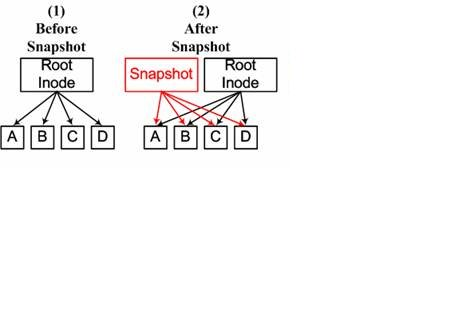
\includegraphics[scale=1.0]{pics/wafl1.eps}
\end{center}
\vspace*{\fill}


\subsection{Filesystem backup}
Example: WAFL (Write Anywhere File Layout)
\vspace*{\fill}
\begin{center}
	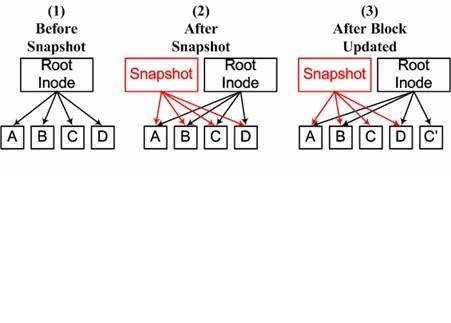
\includegraphics[scale=1.0]{pics/wafl2.eps}
\end{center}
\vspace*{\fill}


\subsection{Filesystem backup}
Example: WAFL (Write Anywhere File Layout)
\vspace*{\fill}
\begin{center}
	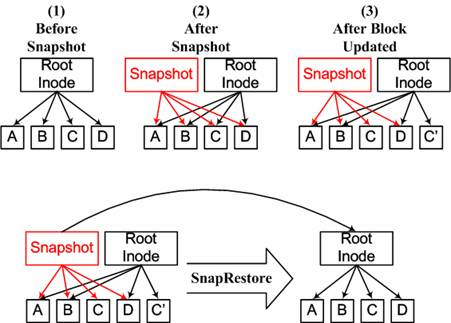
\includegraphics[scale=1.0]{pics/wafl.eps}
\end{center}
\vspace*{\fill}


\subsection{Filesystem backup}
Example: ZFS snapshots
\begin{itemize}
	\item ZFS uses a copy-on-write transactional object model (new data does
		not overwrite existing data, instead modifications are written to a
		new location with existing data being referenced), similar to WAFL
	\item a snapshot is a read-only copy of a file system (cheap and near
		instantaneous, due to CoW)
	\item initially consumes no additional disk space; the writable filesystem
		is made available as a ``clone''
	\item conceptually provides a branched view of the filesystem; normally
		only the ``active'' filesystem is writable
\end{itemize}

\subsection{ZFS Snapshots}
\smallish
\begin{verbatim}
$ pwd
/home/jschauma
$ ls -l .z*
ls: cannot access .z*: No such file or directory
$
\end{verbatim}
\Normalsize

\subsection{ZFS Snapshots}
\smallish
\begin{verbatim}
$ pwd
/home/jschauma
$ ls -l .z*
ls: cannot access .z*: No such file or directory
$ ls -lid .zfs
1 dr-xr-xr-x 3 root root 3 Jan 10  2013 .zfs
$
\end{verbatim}
\Normalsize

\subsection{ZFS Snapshots}
\smallish
\begin{verbatim}
$ pwd
/home/jschauma
$ ls -l .z*
ls: cannot access .z*: No such file or directory
$ ls -lid .zfs
1 dr-xr-xr-x 3 root root 3 Jan 10  2013 .zfs
$ ls -lai .zfs/snapshot
total 13
2 dr-xr-xr-x  4 root     root       4 Feb 28 21:00 .
1 dr-xr-xr-x  3 root     root       3 Jan 10  2013 ..
4 drwx--x--x 37 jschauma professor 88 Feb 24 22:32 amanda-_export_home_jschauma-0
4 drwx--x--x 37 jschauma professor 88 Feb 26 11:47 amanda-_export_home_jschauma-1
$
\end{verbatim}
\Normalsize

\subsection{ZFS Snapshots}
\smallish
\begin{verbatim}
$ pwd
/home/jschauma
$ ls -l .z*
ls: cannot access .z*: No such file or directory
$ ls -lid .zfs
1 dr-xr-xr-x 3 root root 3 Jan 10  2013 .zfs
$ ls -lai .zfs/snapshot
total 13
2 dr-xr-xr-x  4 root     root       4 Feb 28 21:00 .
1 dr-xr-xr-x  3 root     root       3 Jan 10  2013 ..
4 drwx--x--x 37 jschauma professor 88 Feb 24 22:32 amanda-_export_home_jschauma-0
4 drwx--x--x 37 jschauma professor 88 Feb 26 11:47 amanda-_export_home_jschauma-1
$ cd .zfs/snapshot
$ echo foo > amanda-_export_home_jschauma-0/oink
-ksh: amanda-_export_home_jschauma-0/oink: cannot create [Read-only file system]
$ ls -laid . /
2 dr-xr-xr-x  4 root root    4 Feb 28 21:00 .
2 drwxr-xr-x 26 root root 4096 Jan 27 11:44 /
\end{verbatim}
\Normalsize

\subsection{ZFS Snapshots}
\smallish
\begin{verbatim}
$ pwd
/home/jschauma/.zfs/snapshot
$ ls -lai amanda-_export_home_jschauma-0 >/tmp/a
$ ls -lai amanda-_export_home_jschauma-1 >/tmp/b
$ diff -bu /tmp/[ab]
--- /tmp/a	2014-03-01 22:55:49.000000000 -0500
+++ /tmp/b	2014-03-01 22:55:59.000000000 -0500
@@ -35,7 +35,7 @@
 57723 drwx------  3 jschauma professor         6 Dec 31 15:08 .subversion
 49431 -rw-------  1 jschauma professor         6 Dec 22 12:25 .sws.pid
    20 drwx------  2 jschauma professor         3 Jan 26 10:30 .vim
-61768 -rw-------  1 jschauma professor     14538 Feb 24 22:32 .viminfo
+61775 -rw-------  1 jschauma professor     14557 Feb 26 09:23 .viminfo
   173 -rw-------  1 jschauma professor      4355 Sep 17  2012 .vimrc
 45744 -rw-r--r--  1 jschauma professor         0 Jul 28  2013 .xsession-errors
    21 drwxr-xr-x  3 jschauma professor         6 Apr  4  2010 CS615A
$
\end{verbatim}
\Normalsize

\subsection{Summary}
\begin{itemize}
	\item backups are most commonly done as incrementals
		of a filesystem, mountpoint, or directory hierarchy
	\item consider (long-term) storage:
		\begin{itemize}
			\item media and location
			\item increased storage requirements
			\item privacy and safety of the data
		\end{itemize}
	\item self-service restores and filesystem snapshots
	\item backups need to be:
		\begin{itemize}
			\item regular, frequent, automated
			\item invisible
			\item verifiable
		\end{itemize}
\end{itemize}

\subsection{Summary}
\vspace*{\fill}
\begin{center}
	
\includegraphics[scale=0.8]{pics/schrodinger.eps}
\end{center}
\vspace*{\fill}

\subsection{Reading}
Hurricane Sandy
\begin{itemize}
	\item \verb+http://is.gd/aaxzvI+
	\item \verb+http://is.gd/Y75pEA+
	\item \verb+http://is.gd/32Az7y+
	\item \verb+http://is.gd/FhAuFZ+
\end{itemize}

\subsection{Reading}
Backups with {\tt dump(8)} and {\tt restore(8)}:
\begin{itemize}
	\item \verb+dump(8)+ and \verb+restore(8)+
	\item \verb+http://is.gd/bXG9of+
\end{itemize}
\vspace{.5in}

Filesystem snapshots:
\begin{itemize}
	\item \verb+https://en.wikipedia.org/wiki/Snapshot_(computer_storage)+
	\item \verb+https://en.wikipedia.org/wiki/Time_Machine_(Apple_software)+
	\item \verb+http://comet.lehman.cuny.edu/jung/cmp426697/WAFL.pdf+
	\item \verb+http://www.cs.tau.ac.il/~ohadrode/slides/WAFL.pdf+
\end{itemize}
\vspace{.5in}
Book: \verb+http://www.oreilly.com/catalog/unixbr/+

\end{document}
